\chapter{Design}
\label{cha:Design}

This chapter will discuss and overview of the proposed attack and the elements that are required.

\section{Overall attack design}

The attack on Trustwords involves generating "near-collision" keys. 
This will attempt to provide the base to answer Research Questions \ref{goal:numberOfTrustwords}, \ref{goal:complexity} and \ref{goal:hardwareRequired}.

Near-collision keys are keys that are deemed a match by the phonetic similarity metric (More on this aspect in the following sections). A similarity metric is an algorithm designed to determine if two words are phonetically a match. For example, the words "THEIR" and "THERE" will be a match whereas the words "DARK" and "PRINCIPLE" are not phonetically matching.

As each combined key in Trustwords is an exclusive-or of both sides public key (Figure \ref{fig:xor_trustwords} shows this process) the attack is target to a single pair of users and will require recomputation for every attack target. This will be considered when discussing the attack feasibility. Each pair is also split into a "Uncontrolled" and "Controlled" key. Uncontrolled is the reciever of the communication, and, thus, we cannot control their key. The Controlled key is the one we are attempting to impersonate, and it is assumed that we have the ability to replace the Controlled key with our malicious option. These descriptions will be the terminology used throughout the paper. However, it should also be considered that the uncontrolled and controlled can be swapped around with the ability to compute both directions. Thus, resulting in the possibility to intercept both directions of communication. This, however, will require performing the attack separately for both directions.

\begin{figure}[h!]
    \centering
    $KeyFingerprint_{1} \oplus KeyFingerprint_{2} = TrustwordsFingerprint$
    \caption{Creation of the combined Trustword fingerprint}
    \label{fig:xor_trustwords}
\end{figure}

When attacking the respective similarity metric will be used to compute a list of possibilities for each position in the combined fingerprint.

Figure \ref{fig:nearMatch} shows the process of generating a sub section of the combinations. A list of each words matches are generated and then the total number of permutations are generated overall.

\begin{figure}[h!]
    \centering
    \begin{BVerbatim}[commandchars=\\\{\}]
        \centering
\textbf{ CHOKE BLUSHING FRIGHTENING HAND}
    \end{BVerbatim}
    \\
    \verb|COKE                           |
    \\
    \verb|SMOKE                          |
    \\
    \hspace{1cm}



    \verb|CHOKE                          |
    \\
    \begin{BVerbatim}[commandchars=\\\{\}]
\textbf{COKE BLUSHING FRIGHTENING HAND}
    \end{BVerbatim}
    \\
    \verb|SMOKE                          |
    \\
    \hspace{1cm}


    \verb|CHOKE                          |
    \\
    \verb|COKE                           |
    \\
    \begin{BVerbatim}[commandchars=\\\{\}]
        \centering
\textbf{ SMOKE BLUSHING FRIGHTENING HAND}
    \end{BVerbatim}
    \caption{Visualization of the generation of near matches}
    \label{fig:nearMatch}
\end{figure}

To generate an actual list of fingerprints to search for, the near collision words are converted back into hexadecimal and XORed with the uncontrolled key. The provides the impersonated key that will produce the desired combined near-collision. Completing this for all of the near-collision permutations will produce a list of fingerprints that can be inserted into a tool designed to hash keys and search for targets. This aspect of using a large list to search for keys massively reduces the complexity of the search.

In summary the, attack steps are:

\begin{enumerate}
    \item Compute all possible matches using a similarity metric on all words in a dictionary (Only needs performing once).

    \item Select a target and allocate "Uncontrolled" and "Controlled" key identification.
    
    \item Calculate all permutations of near-collisions for the key pair and produce a list of similar key fingerprints.
    
    \item Use list of similar keys in mass computation of keys to find near-collision keys.

\end{enumerate}

\section{Similarity metrics}
\label{sec:metrics}
One of the first requirements for the attack is quantifying "phonetic similarity". This section is looking to provide an answer for the Research Question \ref{goal:phoneticSimilarity}. There are many algorithms currently available to provide this functionality. This section will describe algorithms alongside the reasons they were selected for assessment later in the project.

\subsection{Soundex}
One of the earliest example of a phonetic algorithm is known as Soundex. It is one of the most famous algorithm due in part to its implementation into major database clients like MySQL\cite{mysql_soundex}, Oracle\cite{moved_2005} and PostgreSQL\cite{postgresql}. Originally designed for indexing names by phonetics alongside spelling mistakes due to transpositions in letters. Therefore, due to it being based on the phonetic features, it is highly suitable for this project's use-case. 

Soundex produces a four digit code for each word assessed.
The first letter of the word is retained alongside the removal of all of a, e, i, o, u, y, h and w. The remaining letters are then mapped to numbers\footnote{Further steps are performed on the code, as the technical details do not add anything to the discussion, the steps of the algorithm can be found in Appendix TODO.}. These mappings are displayed in Figure \ref{fig:soundexMap}.

\begin{figure}[h!]
    \centering
    \begin{BVerbatim}
b, f, p, v               1
c, g, j, k, q, s, x, z   2
d, t                     3
l                        4
m, n                     5
r                        6
    \end{BVerbatim}

    \caption{Soundex mappings of letters to numbers}
    \label{fig:soundexMap}
\end{figure}

\subsection{Soundex Issues}
\label{sec:soundexIssues}

Due to the fixed length and limited digit set the initial concerns from this design is the limited number of combinations. There are a total of 5616 codes due to 26 initial letters and three digits of 6 values ($26 * 6^3$).
The limited combinations will result in matches of a limited quality. This will require consideration later in the project.

Further issues posed in \cite{patman2001soundex} are discussed below and show the further deficiencies of Soundex in a dictionary word matching context. 

\begin{enumerate}
    \item \textbf{Dependency on the first letter:} Soundex cannot match words together if their first letters are different, meaning for example the words "KORBIN" and "CORBIN" will never be matched.

    \item \textbf{Silent consonants.} Soundex does not have logic embedded to deal with silent consonants.

    \item \textbf{Poor precision.} Due to the previously discussed point of a small code space. \cite{patman2001soundex} re-iterates this point but in the context of name matching where Soundex's poor performance was demonstrated. Soundex only gained and overall accuracy 36.37\% when matching names within a provided database.
\end{enumerate}

However, even with Soundex's fallbacks its algorithmic simplicity and popularity allows it to still remain relevant in this application.

\subsection{NYSIIS}
The New York State Identification and Intelligence System (NYSIIS) phonetic code was created for use matching the phonetics of American names. It was created due to the presence of hispanic names in the American based databases (this was an aspect Soundex was known to have low accuracy with). However, due to it having embedded rules to handle word phonetics it would, again be applicable in this application.

It also allows for variable length codes and, thus, allows the applicability of the application to increase due to it not confronting the limited code issue of Soundex. It was in use right up the end of 1998 within various US Government departments. Due to this prolific stature and proven track record it was deemed suitable as one of the selected similarity metrics.

\subsection{Metaphone}
Metaphone was invented by Lawrence Philips in 1990\cite{philips1990hanging} in response to the deficiencies in Soundex. It improves on Soundex by including information around inconsistency and variation in English spelling in an attempt to create a more accurate phonetic representation. Metaphone is arguably on the same level of ubiquity as that of Soundex with it finding itself implemented in languages such as PHP\cite{php}. 

Further work would involve the implementation of newer versions of Metaphone. Double Metaphone (2000) and Metaphone 3 (2009) that claim to improve over the original version due to further research performed by Philips. The original version was chosen due to its historical and widespread usage.

\subsection{Levenshtien Distance}
Levenshtein distance is a string metric designed to measure the 'distance' between two strings. It is simply the number of single-character edits (insertions, deletions or substitutions) required to reach the other string. Edit distance is not technically designed as a phonetic algorithm, but due to similar-sounding words often being spelt in similar ways\cite{hettiarachchi2012sparcl} Levenshtien distance was deemed another suitable metric.

An example distance between \verb|trace| and \verb|place| would be the substitutions of the first to letters, from \verb|tr| to \verb|pl| meaning the two strings have a Levenshtein distance of 2.

\subsection{Phonetic Vectors}
Phonetic Vectors is the unique addition to the chosen set. Created by Allison Parrish in 2017\cite{parrish2017poetic}, Phonetic vectors is as the name suggests the vectorization of a words phonetics. This allows a words phonetics to be represented in vector space.

Phonetic features are used in this work as a way to compare the similarity of a words phonemes. Phonemes are the phonetic elements that construct a word. For example the word "RING" translated into the phonemes \verb|/R IH NG/|. 

Extensive prior work has gone into producing models of features that map to phonemes. \cite{chomsky1968sound}\cite{ladefoged1969measurement}\cite{bradlow2010perceptual}. Features, therefore, are an attempt at mapping the varying and inconsistent rules around pronunciation of the English language. The vectors were created using lists phonemes from the CMU Pronouncing Dictionary and mapping them to possible features.

\begin{table}[!htb]
    \tiny
    \begin{minipage}{.33\linewidth}
        \centering
        \begin{tabular}{ll}
            Phone & Features \\
            \hline
            AA & bck, low, unr, vwl \\
            AE & fnt, low, unr, vwl \\
            AH & cnt, mid, unr, vwl \\
            AO & bck, lmd, rnd, vwl \\
            AW & bck, cnt, low, rnd, smh, unr, vwl \\
            AY & cnt, fnt, low, smh, unr, vwl \\
            B & blb, stp, vcd \\
            CH & alv, frc, stp, vls \\
            D & alv, stp, vcd \\
            DH & dnt, frc, vcd \\
            EH & fnt, lmd, unr, vwl \\
            ER & cnt, rzd, umd, vwl \\
            EY & fnt, lmd, smh, unr, vwl
        \end{tabular}
    \end{minipage}%
    \begin{minipage}{.33\linewidth}
        \centering
        \begin{tabular}{ll}
            Phone & Features \\
            \hline
            F &  frc, lbd, vls \\
            G &  stp, vcd, vel \\
            HH & apr, glt \\
            IH & fnt, smh, unr, vwl \\
            IY & fnt, hgh, unr, vwl \\
            JH & alv, frc, stp, vcd \\
            K &  stp, vel, vls \\
            L &  alv, lat \\
            M &  blb, nas \\
            N &  alv, nas \\
            NG & nas, vel \\
            OW & bck, rnd, smh, umd, vwl \\
            OY & bck, fnt, lmd, rnd, smh, unr, vwl
        \end{tabular}
    \end{minipage} 
    \begin{minipage}{.33\linewidth}
        \centering
        \begin{tabular}{ll}
            Phone & Features \\
            \hline
            P & blb, stp, vls \\
            R & alv, apr \\
            S & alv, frc, vls \\
            SH & frc, pla, vls \\
            T & alv, stp, vls \\
            TH & dnt, frc, vls \\
            UH & bck, rnd, smh, vwl \\
            UW & bck, hgh, rnd, vwl \\
            V & frc, lbd, vcd \\
            W & apr, lbv \\
            Y & apr, pal \\
            Z & alv, frc, vcd \\
            ZH & frc, pla, vcd \\
        \end{tabular}
    \end{minipage} 
    \caption{Phonemes to feature mapping table}
    \label{tab:features}
\end{table}

Table \ref{tab:features} contains the mappings used in \cite{parrish2017poetic} to create the phonetic feature lists.
Using this with all 133,852 entries in version 0.7b of the CMU Pronouncing Dictionary, 949 unique properties were produced overall. The author then performed principal components analysis\footnote{Details regarding this process is outside the scope of the project. Please, however, if interested please refer to this resource for more information: \url{http://setosa.io/ev/principal-component-analysis/}} on the unique properties to reduce them down to 50.

This metric allows for a unique set of actions to be performed on the phonetic output. Not only does this metric allow the user to measure \textit{dissimilarity} (opposed to the similar-or-not method of the alternatives) the continuous nature of the value allows mathematical operations to be performed on the output. An example shown in \cite{parrish2017poetic} was the addition of word vectors.

\begin{table}[!htb]
    \centering
    \begin{tabular}{cll}
        No & Operation & Result \\
        \hline
        1  & $Vec(\verb|sub|) + Vec(\verb|marine|)$ & \verb|submarine| \\
        2  & $Vec(\verb|miss|) + Vec(\verb|sieve|)$ & \verb|missive| \\
        3  & $Vec(\verb|fizz|) + Vec(\verb|theology|)$ & \verb|physiology| \\
    \end{tabular}
    \caption{Examples of vector addition}
    \label{tab:vectorAdd}
\end{table}

For example, the addition of vectors can be seen in Table \ref{tab:vectorAdd}. This works for any mathematical operation with multiplication allowing the 'tinting' words with a theme.

The ability to perform operations and measure dissimilarity allows for a plethora of applications. One possible application of note would be the creation of a wordlist where the phonetic difference (vector distance) is maximized. This, if the vector mappings are an accurate representation could allow a creation of a phonetically distinctive wordlist. This will be discussed further at a later stage of the report.

\section{Alternative Similarity Metrics}

\subsection{Match Rating Approach}
Matching Rating Approach (MRA) is another algorithm designed to match names within a database, therefore, its operation can be grouped with that of NYSIIS and Soundex. MRA was discarded as an option. This is because of the lack of known utilization in any substantial real world use-cases alongside its similarity to more well established algorithms of Soundex and NYSIIS.

Further work could include the comparison of this algorithm  to similar alternatives in phonetically matching of words to quantify performance. This will be discussed further in the evaluative sections of the report.

\subsection{Caverphone}
Another notable alternative solution is that of Caverphone that was designed in New Zealand. Caverphone as is the case with the vast majority of phonetic algorithms was designed for use with name matching. Caverphone was not chosen to similar reasons to that of MRA alongside its optimization for accents in location of New Zealand it was conceived in. Therefore, the low level of utilization alongside the unique design features that suggest it may not be suited for this application. This has, however, not be assessed empirically and thus would be a candidate for further work.

\begin{table}[h!]
    \centering
    \begin{tabular}{ll}
        Metric & Output \\
        \hline    
        Soundex & T614 \\
        NYSIIS & TRAVAL\\
        Metaphone & TRFL\\
        Caverphone & TRF111\\
        MRA & TRVL
    \end{tabular}
    \caption{The various phonetic encodings of the word "Travel"}
\end{table}

\section{Design of GreenOnion}
\label{sec:greenDesign}
To answer Research Questions \ref{goal:complexity} and \ref{goal:hardwareRequired} fully, it is necessary to implement an actual code base that will be used to generate actual keys. 

Inspiration of the design of this tool was taken from a tool called Scallion\footnote{\url{https://github.com/lachesis/scallion}}. Scallion was designed by Richard Klafter and Eric Swanson and used to demonstrate that 32-bit PGP key ids were insufficient. Keeping with the onion-based theme the proposed tool is known as GreenOnion and is a re-write of the tools structure in C++. This language was chosen due to the well understood efficiency benefits. The proposed tool differs from Scallion most notably in its ability to concurrently search for a large number of keys, GreenOnion improves on this substantially. More implementation and experimental details will be discussed in later chapters.

The tool should take two keys as parameters (Uncontrolled/Controlled) and a chosen similarity metric and produce a list of target keys fingerprints. This list is then used as a search criteria when hashing a checking a large number of keys. In order to utilise the high parallel nature of the GPU to compute the hash of a large number of keys the tool will utilise a GPGPU (General-purpose computing on graphics processing units) framework. The chosen framework was OpenCL due to its support for the chosen language (C++) and platform (Linux). OpenCL allows the creation of code chunks refereed to as "kernels" to be executed concurrently, this will provide a massive speed increase compare to the sequential nature of the CPU. Technical details will be explained further in Chapter \ref{cha:Implementation}.

\section{Experiment Design}
In order to answer some of the research questions empirical evidence is required and, thus, experiments are required. In this section the designs and considerations of the chosen experiments will be discussed.

\subsection{Metric performance}
\label{exp:metric}
In order to answer Research Question \ref{goal:bestMetrics} and reduce the number of metrics to asses in the later rounds, the performance of similarity metrics required comparison. The thinning out of metrics is required due to limited resources and, therefore, possible further work could involve repeating this work with a much more varied selection of metrics. As explained in a previous section (See Section \ref{sec:metrics}) the chosen metrics up for assessment are Soundex, Metaphone, NYSIIS, Levenshtein and Phonetic vectors.

The design for the experiment involves assessing the quality of the metrics matches by having participants rate them on a scale of 1 to 5.

\subsubsection{Matches}
A match for each code based metric (Soundex, Metaphone and NYSIIS) occurs when the codes are identical. However, for the other cases where the difference is variable other ways of defining a match are required.

In the case of Levenshtein values of similarity are discrete due to it being the number of single character edits. Therefore, this requires less deliberation. Match size was used as a way to decide on a cut-off point.

\begin{table}[h!]
    \centering
    \begin{tabular}{ll}
        Metric & Matches \\
        \hline
        Soundex     & 1,527,554 \\
        Metaphone   & 412,916 \\
        NYSIIS      & 188,474 \\
        \hline
        Levenshtein (Distance 1) [L1] & \textbf{97,730} \\
        Levenshtein (Distance 2) [L2] & 1,070,656
    \end{tabular}
    \caption{Levenshtein number of matches comparison}
    \label{tab:matchSize}
\end{table}

As it can be seen from Table \ref{tab:matchSize} the number of matches for L2 is massively larger than all metrics excluding Soundex. As the issues with Soundex have been discussed in previous sections (See Section \ref{sec:soundexIssues}) it can be excluded as an abnormality in this context. Therefore, due to the excessively high value for a L2, L1 was chosen as the Levenshtein cap for defining a match.

Match size was also used to define the cap for the phonetic vectors. This is less distinct that that of Levenshtein due to the continuous nature of the distance between two vectors, however the complexity was reduced by limiting it to increments of 0.5.

\begin{table}[h!]
    \centering
    \begin{tabular}{ll}
        Metric & Matches \\
        \hline
        Soundex     & 1,527,554 \\
        Metaphone   & 412,916 \\
        NYSIIS      & 188,474 \\
        Levenshtein & 97,730 \\
        \hline
        Phonetic Vector (Distance 3.0)  & 14,550 \\
        Phonetic Vector (Distance 4.0)  & 73,962 \\
        Phonetic Vector (Distance 4.5)  & \textbf{216,156} \\
        Phonetic Vector (Distance 5.0)  & 685,516 \\
    \end{tabular}
    \caption{Phonetic vector number of matches comparison}
    \label{tab:vectorMatchSize}
\end{table}

Table \ref{tab:vectorMatchSize} contains the match size comparison for Phonetic vectors distance. Distance 4.5 was chosen as the suitable size due to the total matches fitting well within the other metrics. Distance 4.0 was the other alternative, this was discarded due to its small size. Any metric with a number of matches below 100,000 results in an inadequate number of possible near-collision keys later in the process, a lower number of matches may imply better quality but a balance is required between computational cost and attack quality. This will be discussed in more detail in later chapters.

\newpage

\subsubsection{Comparisons}
Each participant is asked to rate the similarity of a match on a scale of 1 to 5. Figure \ref{fig:phoneticMatch} shows an example match and the connected scale. Users will complete 5 of these comparisons per metric.

\begin{figure}[h!]
    \centering
    \fbox{
        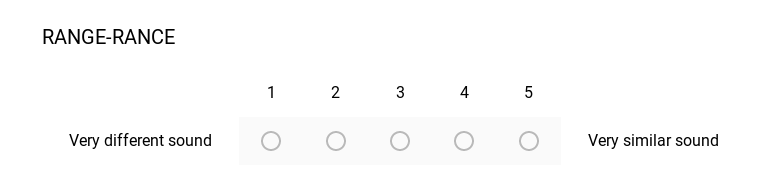
\includegraphics[scale=0.5]{experiment_match.png}
    }
    \caption{Example experiment question}
    \label{fig:phoneticMatch}
\end{figure}

The experiment randomizes the order of these comparisons per session alongside a complete refreshing of matches once per submission. This makes sure selections from the samples are fair and consistent as each user will have a different selection of matches.

\subsubsection{Quality control}
\label{sec:exp1_qualitycontrol}
As the study was being outsourced to Amazon's Mechanical Turk the requirement to check the quality of results is important. Therefore, a couple of additions were provided to check a result's validity.

The first was the addition of 5 "Random matches" questions. These were two random words selected from the dictionary. Therefore, the overall rating of these words should be close to an average of 1. This allows a simple check to see if the user is providing valid results. If their average is too high, the results will be discarded.

\begin{figure}[h!]
    \centering
    \fbox{
        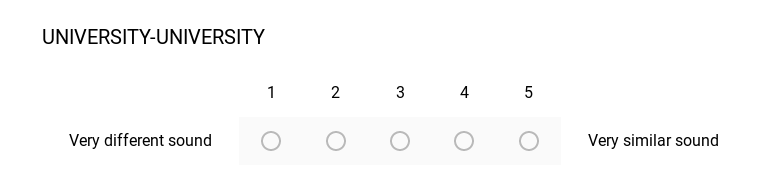
\includegraphics[scale=0.5]{exact_experiment_match.png}
    }
    \caption{Exact experiment attention question}
    \label{fig:exactMatch}
\end{figure}

Alongside this, was the addition of two questions comparing exactly the same word. As both words are the same the result should always be a full 5/5 rating, any results without a full rating will be discarded. Figure \ref{fig:exactMatch} contains one example of the attention questions used to filter inaccurate results.

The final check to ensure the validity of results is a check for native 
English fluency. Having non-native English speakers complete the 
experiment has the possibility to introduce inconsistencies into the 
data and, therefore, needs to remain controlled. To achieve this a 
preliminary MTurk study will be run to ask users for their perceived 
English fluency on a scale of 1 (Basic Understanding) to 5 (Native). 
Workers with an answer of 5 will be provided with a 
Qualification\footnote{\url{https://blog.mturk.com/tutorial-understanding-requirements-and-qualifications-99a26069fba2}} 
that tags them as defining themselves as native speakers. This is then 
added as a prerequisite when running the experiment. This will insure 
only fully native speakers are being assessed. The possibility of the 
worker falsy stating their level of fluency has also been considered. 
However, as the worker does not know the purpose for this initial study,
thereby providing inaccurate results has no real valid motive for the 
worker.

\subsubsection{Statistical}
\textbf{TODO}

\subsubsection{Considerations}
\label{sec:exp1_considerations}
This section will discuss the considerations required when interpreting the results of the study.

The first consideration is the way the words are compared. Due to the channel of authentication being phone based the comparison of words will be a mixture of auditory and textual. This is because a user needs to match a words sound to the one displayed on their device. In the case of this experiment the users are asked to compare the sound of two word that are visually displayed to them. Therefore, this experiment does not fully capture the targeted scenario. This was decided partly to aforementioned lack of resources. The main design of the experiment was to provide a simple way to cull the large number of metrics. The initial choice of five metrics discussed in Section \ref{sec:metrics} was to be followed by a more empirical decision. Further work, therefore, could improve by producing more conclusive results on the performance of the metrics.

Another consideration is the demographics of people accessible on Mechanical Turk. A comprehensive and still active survey run by D Difallah \textit{et al.} \cite{difallah2018demographics} shows that MTurk workers are younger and have a larger household income than that of the US population. This has to be taken into consideration when interpreting the results because it will inherently introduce a bias. This is due to the assumptions that an increase in age provides a better understanding of more obscure words, and, therefore, a better representation of the metrics performance over the entire dictionary.

\newpage

\subsection{Trustword Attacks}

The final experiment required to answer the Research Question \ref{goal:attackPercentage} will simulate attacks on participants. The user will be presented with the same design as presented in the \pep Android application (See Section \ref{sec:pep}).

\begin{figure}[h!]
    \centering
    \fbox{
        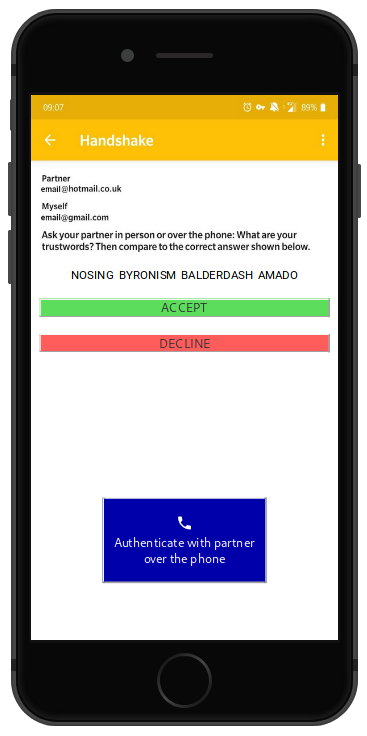
\includegraphics[width=\textwidth]{experiment/trustword_attack.png}
    }
    \caption{Experiment UI}
    \label{fig:expID}
\end{figure}

Figure \ref{fig:expID} shows the design of the experiments front end. As can be seen by comparing it to Figure \ref{fig:trustwords} it has been designed to be a close as possible to the actual application. Users will click the blue button to simulate the authentication ceremony over the phone. A text-to-speech system will then read a set of words and the user should accept if they match and decline if they don't.

\subsubsection{Design}

Due to the scarcity of attacks in a real-world setting users will are often complacent about their occurrence. Therefore, in this experiment attacks only occur 30\% of the time. This is a much higher value than in a real-world setting, but it is a balance between resources and realistic design. Alongside, this the first 5 trials of a new experiment will always be benign. This is to ensure users are lulled into a level of complacency regarding the possibility for an attack.

Certain keys have higher levels of near-collision possibilities than others due to how certain words are deemed similar by the chosen metric. Therefore, this presents the possibility to have keys with a very low number of similar matches. The distribution of these keys will be explained further in Chapter \ref{cha:Experiments}. Therefore, if random sets of words were chosen with no restraints there are attacks presented to the user that in a real setting would be infeasible in this context as they are close to a $2^{64}$ attack (4 Words * 16-bits). Therefore, the experiment will sample from a list of "vulnerable" keys. These are keys that have a number of combinations that allow an attack in a certain timeframe. Furthermore, certain levels of attacks are also simulated. Below are the list of possible attacks:

\begin{itemize}
    \item \textbf{Zero static words} - All words in the set can vary.
    \item \textbf{One static word} - All but the first word can vary.
    \item \textbf{Two static words} - All but the first and last word can vary.
\end{itemize}

The start and ends were chosen as the highest priority words to keep static. This is due to research highlighting on the common habit of users to only check the start and end of a checksum. \cite{cherubini2018towards} shows this by measuring user eye movement and displaying it as a heat map.

\begin{figure}[h!]
    \centering
    \fbox{
        \parbox{\textwidth}{
            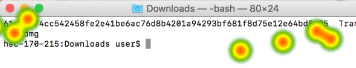
\includegraphics[width=\textwidth]{checksum_check.png}

            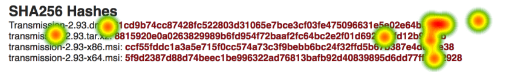
\includegraphics[width=\textwidth]{checksum_check_2.png}
        }
    }
    \caption{Failed verification of an incorrect checksum\cite{cherubini2018towards}}
    \label{fig:heatMap}
\end{figure}

Figure \ref{fig:heatMap} shows the results of a eye tracking experiment where the user failed to detect a mismatching digest. As it can be clearly seen the users never compared the center of the digest. 

However, this may not be applicable in this context due to the user being linearly fed an audio stream that they cannot skip to the start or end. However, we believe that attention will also play a part in defining the most important areas of comparison as the hypothesis is that the users attention will be lower in the middle sections of comparison where it peak at the start and end. All these aspects, however, will require empirical evidence to arrive at a conclusion. Therefore, this consideration will need to be made when assessing the results of the experiment.

These attacks are ascending in complexity. The timeframe for finding a match was decided as 7-days on with attack strengths of 1 GPU/day, 10 GPU/days and 100 GPU/days on a mid range GPU (AMD RX 480 was the example in experiments). 

\begin{table}[h!]
    \centering
    \begin{tabular}{lll}
        GPU/days & No of combinations required & Attack Type \\
        \hline
        1       & 15250   & Zero static\\
        10      & 1525    & One static\\
        100     & 152     & Two static\\        
    \end{tabular}
    \caption{Summary of attack requirements}
    \label{tab:attackReq}
\end{table}

Table \ref{tab:attackReq} contains a summary of the different level of attacks and their respective restrictions. More combinations makes the attack search quicker as there are more possibilities.

Any key that exceeds this criteria is deemed as vulnerable is one of the three attack contexts. A list of these vulnerable keys are sampled from when an attack is simulated. The percentage of vulnerable keys will be explored in Chapter \ref{cha:Experiments}.

\subsubsection{Quality control}
As the previous experiment, participants will be sourced from MTurk. Therefore, again, quality control is and aspect that requires consideration. As with the previous study, initially screened native speakers will be used. The same process will be performed to recruit suitable workers. Two metrics will be used to detect invalid results. Audio button clicks and overall time taken. 

Audio buttons clicks is the number of times the blue \textit{"Authenticate with partner over the phone"} button in Figure \ref{fig:expID}. If there are rounds without button clicks, this is a sign of non-attentive users. The design choice was made to keep this as a result filter, as preventing non-clicks would be a trivial task. This provides a way to detect and discard click-throughs\footnote{Workers that aim to complete the task as fast as possible, with no regard for the quality of responses}. 

Overall time taken is as the name suggest a recording of the time taken to complete the entire experiment. If users complete the experiment in an abnormally small amount of time it can be used as another detection for invalid responses. Anything below a certain threshold will be discarded.

\subsubsection{Statistical}
\textbf{TODO}

\subsubsection{Considerations}
\textbf{TODO}

Demographics of MTurk workers (Discussed in the previous section)